\chapter{on diversity}
 Morrison et al.\cite{populationDiversity} described the pair-wise Hamming distance as one of the most commonly used measures of distance in genotypic space, and is what will be used here to calculate a populations diversity as one scalar metric. In implementation, this algorithm\ref{eq:Hamming} is counting the number of genomes in all pairs of genotypes which is not identical. Another description is the edit distance between two binary genomes. 


where y is a genotype, P is the population size and L is the number of genomes in a genotype.

A problem with using a pairwise Hamming distance is that the number of computations is quadratic with the size of P. Meaning the computational time is quite long, but since this metric is only to be calculated once when experimentation is completed, the restriction this puts on the experiment is negligible. However, a suggested alternate way of calculating population diversity on the basis of edit distance is by calculating the mean edit distance from every genotype to a \textit{centroid} genotype where the centroid is the average genotype in a population, and its i-th element can be given as  
\begin{equation}
    \label{eq:centroid}
    \varphi_{i}=\tfrac{1}{P}\sum_{j=1}^{P}y_{ji}
\end{equation}
Using this vector that can be calculated linearly with respect to P, a diversity metric \(\Delta\) can be calculated as 
\begin{equation*}
    \Delta = \tfrac{1}{P}\sum_{j=1}^{P}\sum_{i=1}^{L}\left | \varphi_{i}-y_{ji} \right |
\end{equation*}

\begin{equation}
    \label{eq:homemade diversity}
    \Delta = \tfrac{1}{{P}}\sum_{j=1}^{P}\sum_{i=1}^{L}\left | (\tfrac{1}{{P}}\sum_{{j}'=1}^{P}y_{{j}'i})-y_{ji} \right |
\end{equation}
While it is obvious that calculation time grows linearly for larger population sizes and the computational requirements for large experiments are greatly reduced, the pair-wise Hamming distance is a tried and tested diversity metric, and is what will be used to describe the change in diversity between generations and algorithms. 

%%%%%%%%%%%%%%%%%%%%%%%%%%
\begin{equation}
    \label{eq:linearHamming}
    \sum_{j=1}^{j=P-1}\sum_{{j}'=j+1}^{{j}'=P}\sum_{i=1}^{i=L}\left |y_{ij}-y_{i{j}'}\right | = \sum_{i=1}^{L}\left [ \left (  P-\sum_{j=1}^{P}y_{ji} \right )\sum_{j=1}^{P}y_{ji} \right ]
\end{equation}

%%%%%%%%%%%%%%%%%%%%%%%%%%
\begin{figure}
    \label{fig:diversity_comparison}
    \begin{subfigure}[h]{0.49\linewidth}
        \label{fig:diversity_comparison:Hamming}
        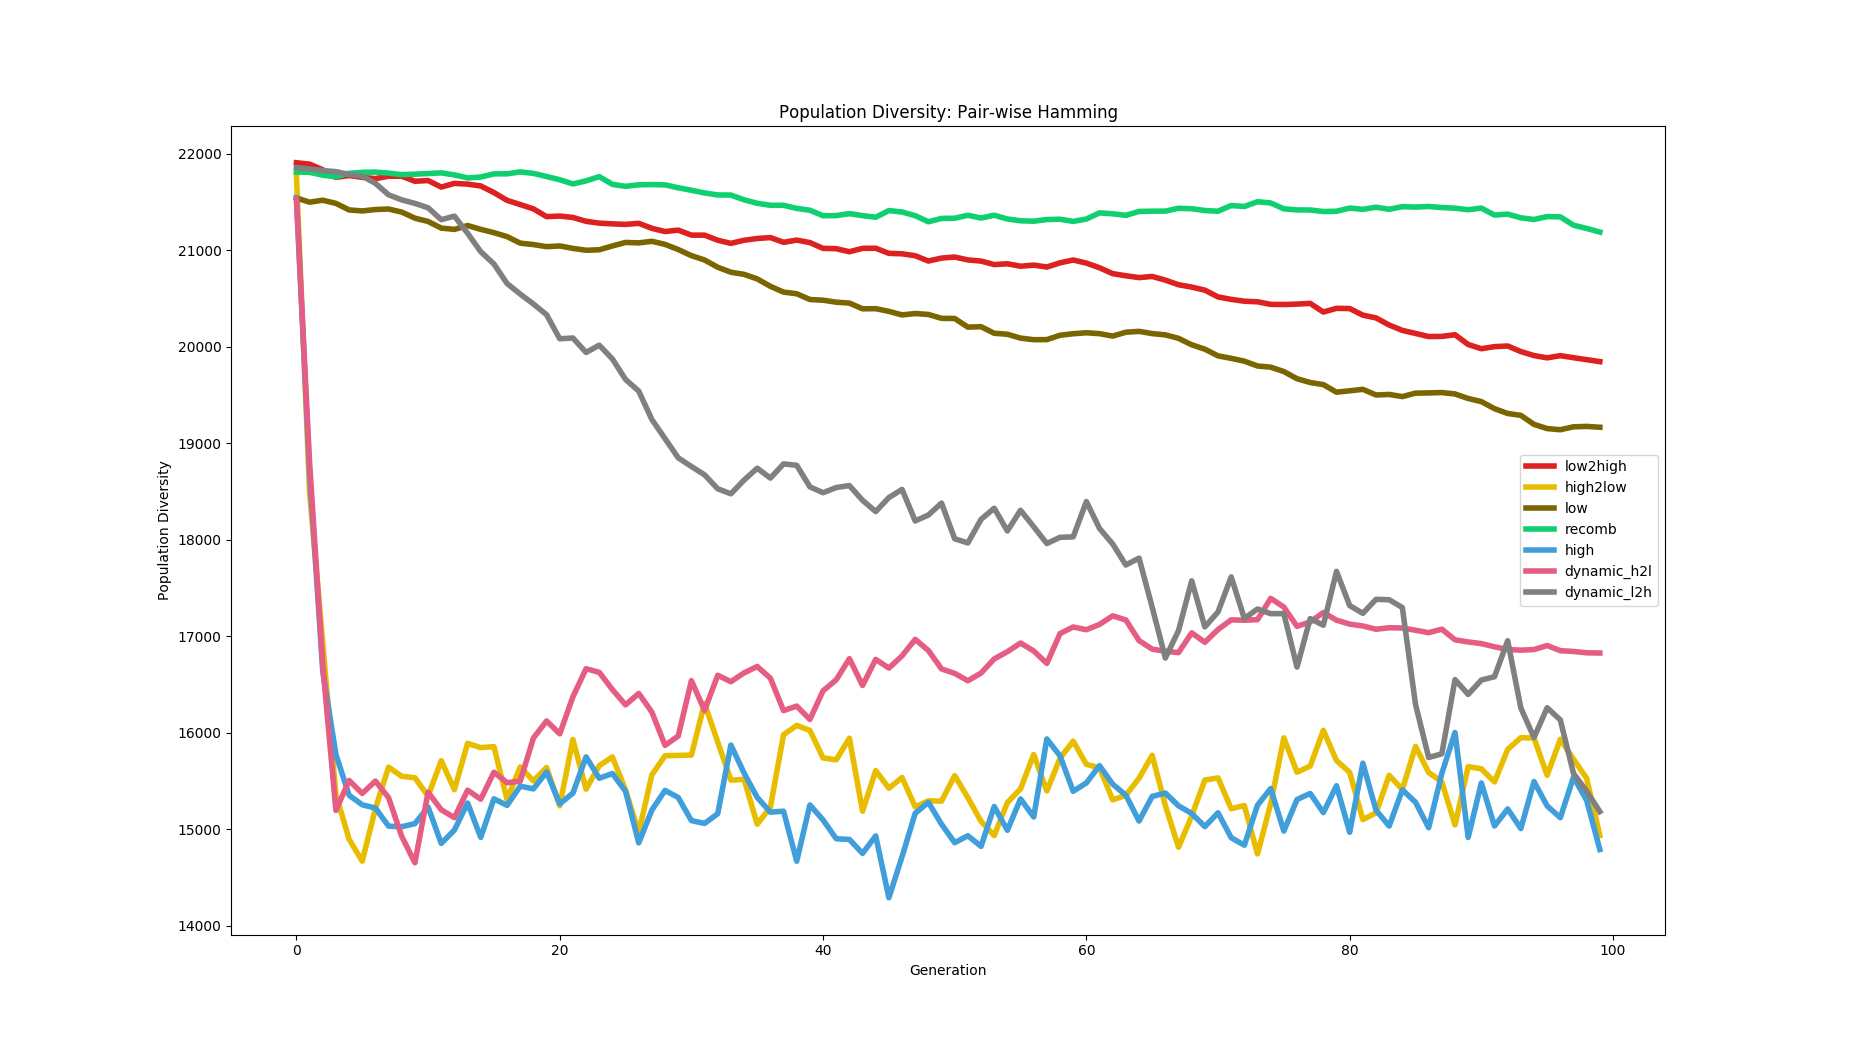
\includegraphics[width=\linewidth]{Chapters/Experiments/search_algo/figures/diversity_showcase_hamming.png}
        \caption{Pair-wise Hamming distance.}
    \end{subfigure}
    \hfill
    \begin{subfigure}[h]{0.49\linewidth}
        \label{fig:diversity_comparison:homemade}
        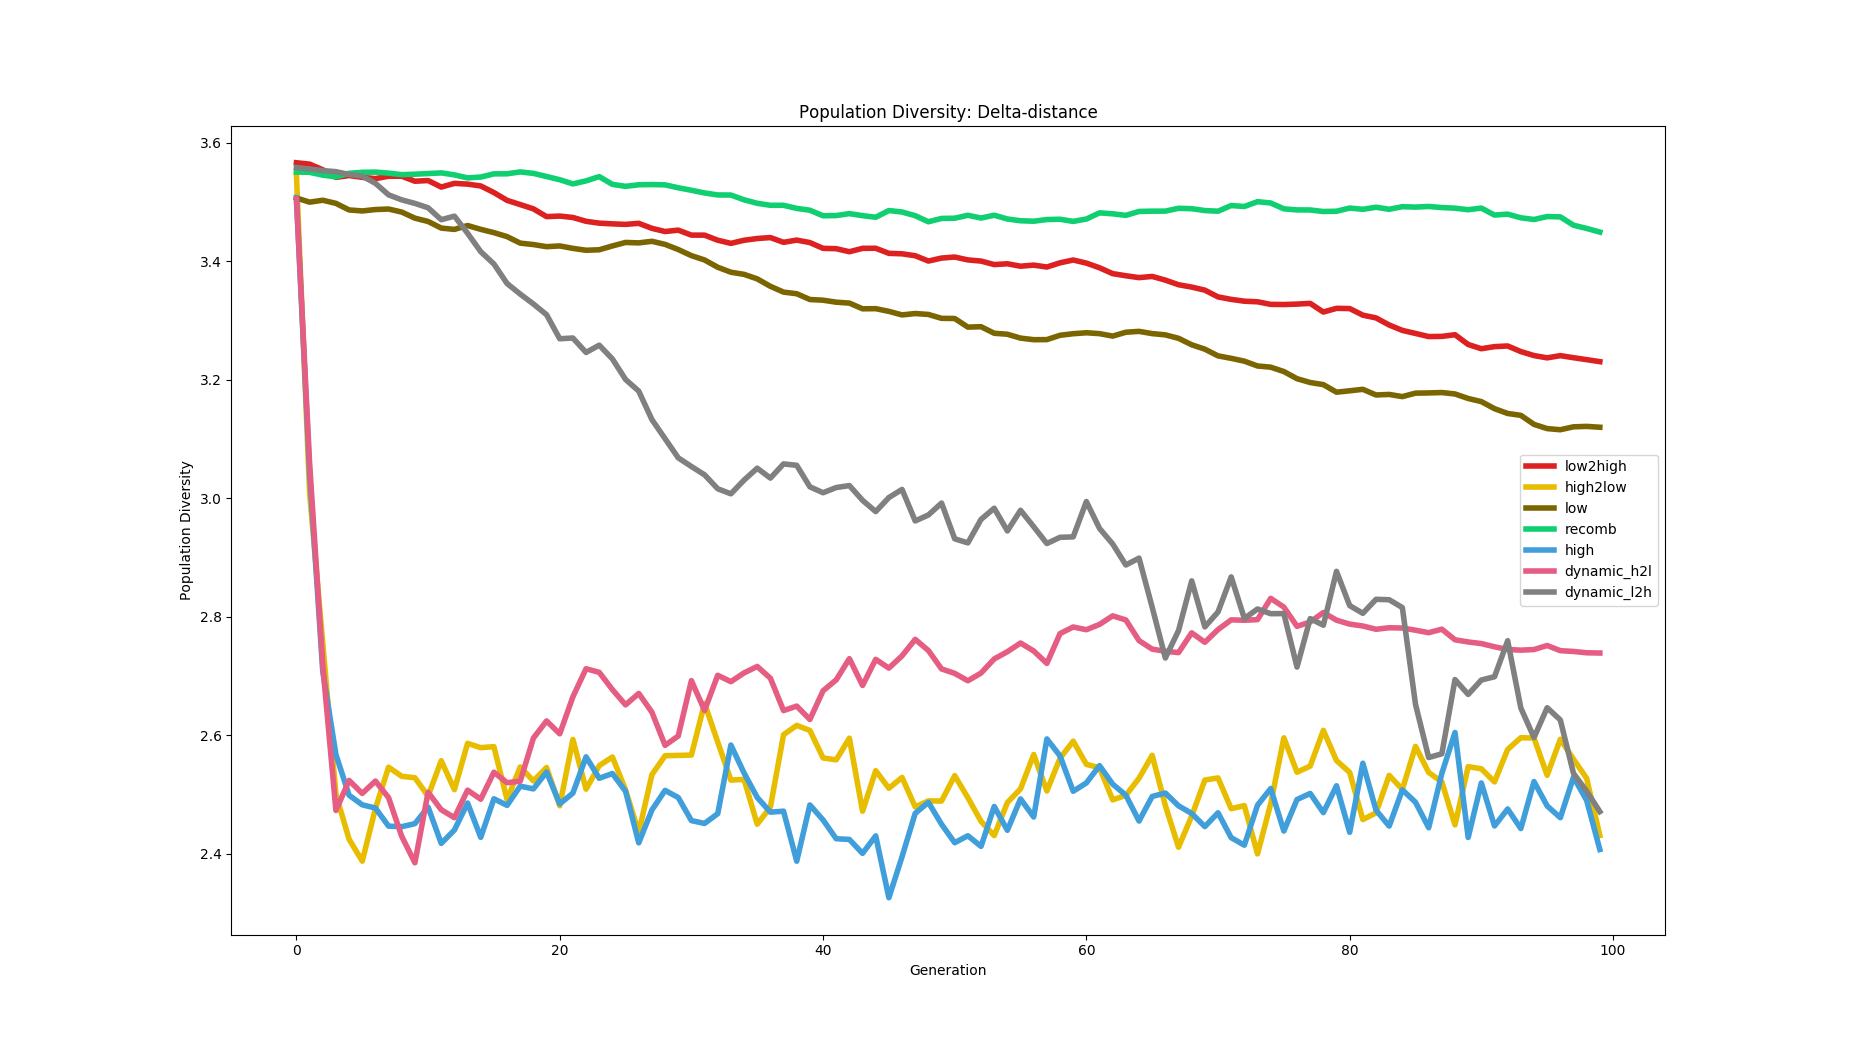
\includegraphics[width=\linewidth]{Chapters/Experiments/search_algo/figures/diversity_showcase_homemade.png}
        \caption{\(\Delta\)-diversity metric}
    \end{subfigure}%
    \caption{A comparison of pair-wise Hamming distance and \(\Delta\)-diversity. The diversity is the average population diversity for each generation during the search for an optimal path for task 1a. Note the similar curves for each algorithm and the scale on the y-axis}
\end{figure}
\chapter{on path size plot}
While algorithms in group 1 and 2 follow their group rule of reaching convergence for high selection pressure, or not converge within 100 generations for the low selection pressures, algorithms 3a and 3b both converge within the 100 first generations. This could be because these searching schemes both are effective ways of optimizing the capacity in paths, or it might be that the average selection pressure within these searches is a selection pressure that works well for this generation limit. We can back up this claim by the fact that algorithms 2a and 2b both converge for task 3 and 4, which for these algorithms and these tasks, have about the same tournament size as the average tournament size in 3a and 3b. 

As a paths size can not change due to mutation, it is reasonable that some of the algorithms with high selection pressure finds optimal sizes which is lower than the average initialized size of 6. This effect could lead to the conclusion that for these tasks, algorithms with high tournament size needs less capacity to solve the task. However, this could be a random effect where some of the initialized paths with fewer modules happened to have a higher fitness. As searches with lower selection pressure all row the average path size or keep it the same, it does not seem that a larger path capacity hurts fitness.
\chapter{}
- Low trains quickly and reaches a performance the same as most of the other algorithms. Few total number of training iterations cause the modules not to overfit mentionably. A population of 64 and termination limit of 100 might not be well suited for this algorithm though. A higher generation limit would give the algorithm a decent chance at finding a optimal path within its population, and a smaller population size together with maybe a higher mutation rate increase the probability of pretrained(MAYBE JUST A SMALLER PATHNET?) modules to be tried in a path before new modules have optimized so much that introducing a old module to a path would reduce fitness below that of the newly trained modules. - Having a high tournament size for the later searches yield higher module reuse than lower tournament sizes, regardless if the previously trained modules were trained using a high or low tournament size. 
\chapter{Conclusion on reuse: removed because of duplication}
When performing ANOVA tests on the amount of module reuse, a test of the null hypothesis yields a P-value not sufficient to reject \(H_{0}\), while adding either 2a or 3b to the test causes \(H_{0}\) to be rejected. While this makes a case for high selection pressure leading to higher reuse, null hypothesis for \(\bar{\mu}_{2_{a}}=\bar{\mu}_{1_{b}}\) can not be rejected, but 2a and 2b is shown to be significantly different from each other. From this, the conclusion drawn is that more experimental runs are needed to be able to say anything meaningful about what causes an increase in module reuse.
\begin{equation*}
    H_{0}:\bar{\mu}_{1_{a}}=\bar{\mu}_{1_{b}}=\bar{\mu}_{1_{c}}=\bar{\mu}_{2_{b}}=\bar{\mu}_{3_{a}}
\end{equation*}
\chapter{Old hypothesis}
The expectations for these experiments were heavily influenced by the results in the first-path experiments. When the training algorithms are viewed in a simplified context of only "exploration vs exploitation", we can place them on a scale between these extremes and discuss expected outcomes from each end of the spectrum. In this context, the Pick+Search learning scheme used in the first-path experiments would fall on the exploitation side.

During a search, a given algorithm reduces the population diversity from a initialized state of high diversity until some optimal path is found. This convergence rate, and therefore also population diversity, is determined by which end of the exploration/exploitation spectrum we select our algorithm from. Since we limit ourselves by only changing the tournament size, we would expect a lower tournament size to lead to a low convergence rate and high diversity. This is a natural assumption to make considering the maximum change that occur in the population from one generation to the next. A tournament search with size two has such a low selection pressure that from one generation to the next, only one instance of genotypic change is applied the the population\footnote{This is when the weakest genotype is replaced by the winner of the tournament}. The number of generations until the population have converged to one optimal path would therefore be higher under such a search than a search where the selection pressure is considerable higher. 

A high selection pressure means strong phenotypes are favoured during the search. The algorithm would after one generation have a significant portion of its population genetically identical, ignoring possible genotypic traits caused by mutations. In the search context of finding an optimal path in a PathNet structure, evaluating a lot of similar paths to rank their fitness would lead to training the same modules multiple times. The next generation would then have a disproportionate fitness scores for some paths which would cause them to have a higher likelihood of winning the next generations tournament, and therefore quickly take control of a population by out performing all other paths. In such a scenario, the population have converged before other paths would have had time to adapt to pretrained modules interfaces, and the advantage PathNet brings with module transferability have been reduced, if not lost.  

For the locked tournament sizes the expectations are that high selection pressure causes high convergence and low module reuse between tasks. The low reuse would again cause more of the total number of modules in the PathNet to be locked after all tasks are learned. What the pressure would mean for validation accuracy is highly dependent on what tasks are learned, and from which domains they are selected. 
The opposite is true for the searches with a small tournament size. The low convergence leads each module to be trained in multiple permutation of PathNet subsets, and therefore also more transferable than modules trained during high selection pressure. If the searches are limited by the number of generations, and not by a threshold training accuracy, it would not be a surprise if the high tournament sizes yields paths with a higher validation accuracy for each task than those searches with low selection pressure. This is because each generation contain more effective training when there are more genotypes in the tournament. Not to be forgotten is the fact that all paths in all generations have the same final task-specific layer.  Since this is shared across all paths, the high tournament sizes leads to orders of magnitude more training in the final layer for high selection pressures. For each generation, the final layer is trained once for each genotype being evaluated. Meaning after a hundred generations, it have been trained 1 order of magnitude more for a search with tournament size of 25 versus a tournament size of 2. 

In addition to the static tournament sizes with a winner-replace-all crossover scheme, a search with recombination is tried together with tournament size three.  This should give a selection pressure even lower than that of tournament size two. From one generation to the next, there is still only one genotypic change in the population, but where the normal tournament search replace the loosing genotype with the winner, a recombination of the two strongest phenotypes replaces the weakest genome\footnote{With some additional mutation}.  Another way to view the step from algorithm 1a to algorithm 1c is one with focus on the genome in the offspring that takes the weaker paths place in the population. Given the recombination scheme, it can be seen as a copy of the tournament winner, but with a strong mutation probability that is scaled down during the search. This down scaling comes from the convergence of the population. When the diversity is reduced, more and more paths will have a similar subset of modules. When selecting two paths with the same modules, the recombination will yield a path identical to both parents. So as a population grows closer to converging to an optimal path, it will consist of similar genomes and each recombination will give offspring closer to the population median than it would in a diverse population. 
In summary, a high tournament size is expected to shift the search algorithm in the direction of high exploitation which in turn should give a high performance on the different tasks. Low tournament sizes gives a high exploration of the different paths possible, which yields modules trained in multiple permutations of PathNet subsets. It is expected that this will lead to more module reuse, and generally have a lower capacity usage than algorithms of high selection pressure. 

It is hard to tell how the validated classification accuracy on the final task will be affected by the different algorithms. As with the previous experiments, the tasks selected might prove to be to simple which would hide much of the potential in transfer learning since a path of average since should be able to learn each task \textit{tabula rasa}.
\chapter{Old metrics}
\subsection{Metrics}
\label{exp2:metrics}

Due to the experiment complexity and number of tunable hyperparameters there are a large number of search effects and attributes that could be investigated, so limitations have been introduced on which metrics are being addressed. 

As with the first-path experiments, module reuse between tasks will be an important metric. This number is highly effected by stochastic processes such as initialization of populations, mutation probability, layer sizes, path sizes and so on, but it is also the most intuitive and clear way to measure the transferability of module knowledge. An assumption used behind this metric is that modules are able to contain some form of "memetic"\footnote{Memetic is used here to describe a quantification of knowledge in the same way "meme" is used by Richard Dawkins\cite{selfishGene} to describe a unit of cultural knowledge, here as a unit of knowledge used to solve a task.} unit knowledge. In this multi-task scenario, reuse can occur across multiple tasks, but focus will here be put on the total number of modules reused instead of separating the reuse across tasks. This is because any effect algorithm choice has on module reuse will be compounded and easier to spot in the total amount of reuse rather than in reuse between tasks.

This reuse can indirectly be seen by viewing the total number of modules used for all tasks. This total capacity use is both a result of the reuse of modules and the path size. Which means capacity could be used as a measure of how "effective" the learning under a search algorithm is. By using few modules in each task and reusing a high number of modules from previous tasks, little new parameter optimization have to be done. This effective parameter use would possibly reduce the overall validation accuracy so in order to visualize the effectiveness of training, total number of training units applied to each module in each path would be a useful metric. 

To confirm the ordering of algorithms on the exploration/exploitation scale, a population diversity metric will be calculated\footnote{See \ref{background:diversity} for more details about how this is computed} for each algorithm. The reduction in this diversity for each generation gives an indication of the convergence-rate of each algorithm. Those of high exploitation will quickly hone in on one genotype and optimize the weights along that path, while algorithms that focus on exploration will explore many more permutations of modules. 

During a search for an optimal path as solution to a given task, the total training effort spent on the task is spread across the modules available for training. This means when the search is terminated and the optimal path have been locked to future back propagation, most of the updated parameters are lost due to the re-initialization of open modules. While total computational efficiency is not something addressed in this thesis, the ratio of used training effort to the total training spent on a task is an interesting metric. This ratio is highly dependent on how quickly a population converges to one optimal path. In scenarios where this occur fairly early on in the lifetime of the search, every subsequent generation performs training where almost all is along the optimal path. We would therefore expect algorithms with a high selection pressure to be placed high in a ranking of useful training. See \ref{exp2:implementation} for description of a training unit. 
